%%%% Small single column format, used for CIE, CSUR, JACM, JDIQ, JEA, JERIC, JETC, TAAS, TACCESS, TACO, TALG, TALLIP (formerly TALIP), TCPS, TEAC, TECS, THRI, TIIS, TISSEC, TIST, TKDD, TMIS, TOCE, TOCHI, TOCL, TOCS, TOCT, TODAES, TODS, TOIS, TOIT, TOMACS, TOMM (formerly TOMCCAP), TOMPECS, TOMS, TOPC, TOPLAS, TOPS, TOS, TOSEM, TOSN, TRETS, TSAS, TSC, TSLP, TWEB.
% \documentclass[format=acmsmall, review=false, screen=true]{acmart}

%%%% Large single column format, used for IMWUT, JOCCH, PACMPL, POMACS, TAP, PACMHCI
% \documentclass[acmlarge]{acmart}

%%%% Large double column format, used for TOG
\documentclass[acmtog,authorversion]{acmart}

%%%% Generic manuscript mode
%\documentclass[manuscript,review,screen]{acmart}
%\setcitestyle{super,sort&compress}


 % For formal tables

 % For algorithms

% Metadata Information


%\acmBadgeL[http://ctuning.org/ae/ppopp2016.html]{ae-logo}
%\acmBadgeR[http://ctuning.org/ae/ppopp2016.html]{ae-logo}

% Copyright
\setcopyright{none}
%\setcopyright{acmlicensed}
%\setcopyright{rightsretained}
%\setcopyright{usgov}
%\setcopyright{usgovmixed}
%\setcopyright{cagov}
%\setcopyright{cagovmixed}

% DOI



% Document starts
\begin{document}
% Title portion
\title{Exchange rate Analysis} 

 \subtitle{TEAM Z}


\author{Philip Wilson}

\author{Nunzio Gatti}

\author{Susmita Gangopadhyay} 

\author{Sumesh Ramachandra}

\author{Bang Du}



\begin{abstract}
An exchange rate is the rate at which one country exchanges currency with another.  In our application we have tried to capture the exchange rate of one country and found out other exchange rates which are most closely correlated with its behaviour.  We have considered G20 countries from a time frame of Dec 1998 to Dec 2017.
\end{abstract}










\maketitle


\section{Github}

\href{https://github.com/sg4g17/Cycle-to-Work}{https://github.com/sg4g17/Cycle-to-Work}
\newline
Our repo is named after our original project name and unfortunately is a  miss leading considering our final project is related to economics.
\section{Introduction}
As team we had first decided on a different topic "Will I live longer if I cycle to work?" . But in the process of trying to collect data it was seen that there was a lot of scientific studies associated with the topic but we struggled to find a way of meaningfully combining different life expectancy models.  Most of the data we found was already clean and we did not have much processing to do\cite{iacono2008access}. We could not find out any scientific method that directly links the factors we were considering(amount of oxygen intake, pollution,BMI etc)to the increase in life expectancy\cite{edwards2014spinning}.Combining all these factors into one prediction model became a challenge.
\newline
So ,after spending almost 4 weeks in trying to collect data we had to shift our focus to some other topic where we could get a significantly high volume of data.  Now we are trying to predict the top three indicators affecting the currency of that country.  After a considerable amount of research We have taken into account the following factors exchange rates, interest rates, employment, population, import, export, GDP and inflation\cite{kuruwitaarachchi2018design}.  The annual factors, like the employment, population, trade networks, GDP and inflation are taken in the time range of 1991-2016.

% Head 1
\section{Problem Statement}
\subsection{High Frequency Exchange Rate Data}
Our aim was to investigate how exchange rates influence each other.  As we were able to gather nearly a 1000 samples we where able to perform a number of different machine learning techniques to perform this analysis.

\subsection{Low Frequency Economic Indicators}
From investigating economic research we were directed towards a number of different economic indicators which are understood to influence a currencies value.  These indicators are only reported on a annual basis and due to a number of factors was only available from 1999 to 2015.  This means we only had 17 samples.  This limited the type of analysis we where able to perform. So we decided to find the economic which where most correlated to the performance of a specific exchange rate. 

\section{Implementation}
\subsection{High Frequency Exchange Rate Data}
\subsubsection{}{Cleaning with python}
\newline
The data that we have collected is from oanda.com, Bank of England and World Bank websites. 
\newline

\iffalse
\begin{figure}[!h]
	\begin{center}
		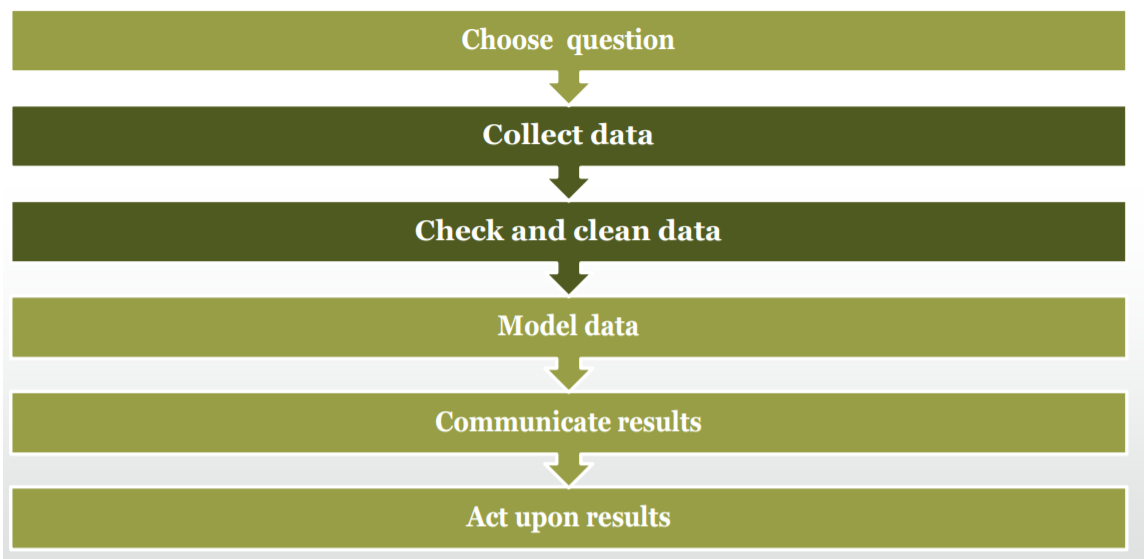
\includegraphics[width=0.40\textwidth]{aa.png}
		\caption{}
		\label{}
	\end{center}
\end{figure}
\fi

First step, Download : For the currency exchange data, it was about weekly average exchange rates from December 1998 to December 2017. We considered all currency of the G20's countries and downloaded them with GBP as the base currency\cite{abbate2018point}. Every file downloaded was made in this way (see Fig\ref{raw_curr}): 

\begin{figure}[!h]
	\begin{center}
		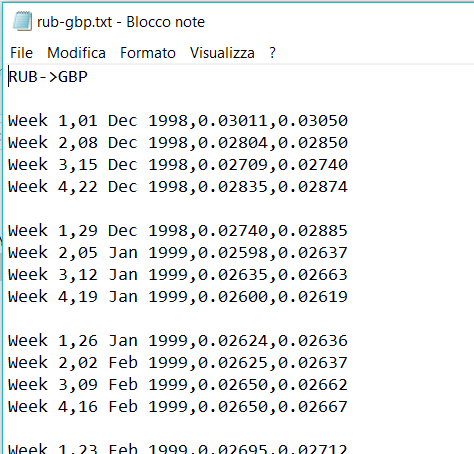
\includegraphics[width=0.40\textwidth]{aaa2.png}
		\caption{Raw currency data}
		\label{raw_curr}
	\end{center}
\end{figure}


For currency exchange data below technique was observed
\begin{itemize} 
\item Size of table : 1240 x 4 columns 
\item Col[0]= Week(1,2,3,4) 
\item Col[1]= Month-Year(i.e may 2002) 
\item Col[2]= Bid ( Bid is the price a buyer is willing to pay for a security) 
\item Col[3]= Ask ( Ask is the price a seller is willing to accept for a security) 
\end{itemize}

Second step, Aggregation : We had 16 files(16 because in the G20 group France, Italy, Germany and European Union has currency Euro).  Using python we gave in input a file formed by 1240(included blank space between rows) x 4 columns and received the output below in Fig \ref{part_proccessed}. 
\newline

\begin{figure}[!h]
	\begin{center}
		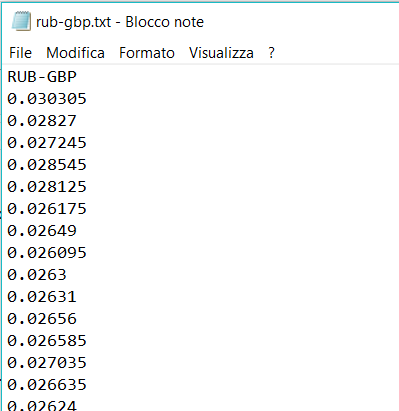
\includegraphics[width=0.40\textwidth]{aaa1.png}
		\caption{Intermediate Processed Data}
		\label{part_proccessed}
	\end{center}
\end{figure}

All spaces were removed using python,  saved in one different file, and an average between bid and ask was calculated.
\newline
Third step, Creation of a complete matrix : We wrote another python script called complete Matrix.py that was used to create all possible currency pair. Remembering that the currency were 16 , we had a output matrix with 16x16 column and 994 rows (see Fig\ref{extrap_ex_data}).

\begin{figure}[!h]
	\begin{center}
		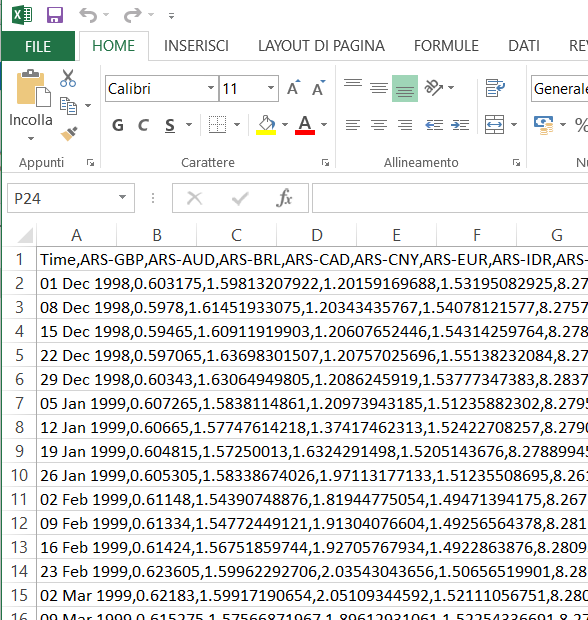
\includegraphics[width=0.4\textwidth]{bbb.png}
		\caption{Extrapolated exchange rate data}
		\label{extrap_ex_data}
	\end{center}
\end{figure}

\subsubsection{Modeling}
The target for this assignment was, given a currency exchange rate as an input, find the \textbf{three} most relevant currency exchanges rates that most influences it. To do that we considered the matrix containing all possible combinations of currency exchanges and we used Matlab for this analysis. We used linear regression technique to create a model to find if there is a clear relationship between one exchange rate and the other G20 exchange rates. We then look to find what are the top 3 currencies that influences the given exchange rate.
\newline
Procedure:
To find the most relevant exchange rates we created a Matlab script using CVX tool. CVX is a modeling system for constructing and solving disciplined convex programs (DCPs)\cite{leung2000forecasting}. 

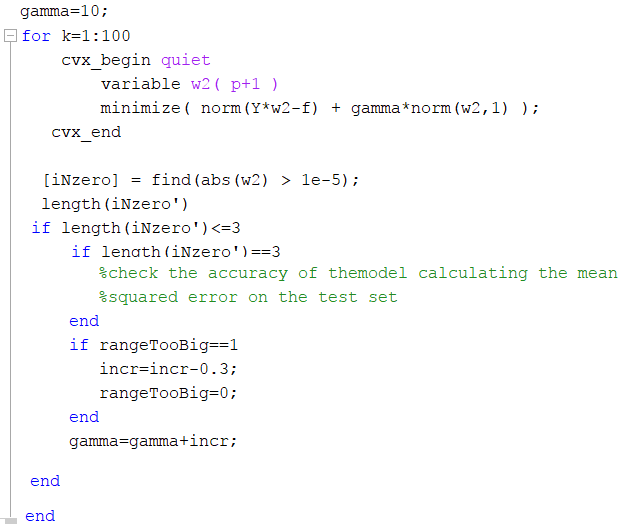
\includegraphics[width=0.4\textwidth]{ccc.png}

Explanation of the procedure : 

\begin{itemize}
\item cvx\_begin : Must be written as the first instruction of a CVX model
\item cvx\_begin quiet : Prevents the model from producing any screen output while it is being solved.
\item cvx\_end : Must be the last instruction of the CVX procedure 
\item variable : It is used to declare the variable, it includes the name of the variable, an optional dimension list, and one or more keywords that provide additional information about the content or structure of the variable.
\item minimise : It is a command used to declare an objective function (can be also maximise) 
N.B. The objective function in a call to minimise must be convex; the objective function in a call to maximise must be concave. In this case Y*w2-f is convex.
\newline
\textbf{Goal :To find the best weight vector that minimises the error }
\item +gamma(w2) : We used gamma for the L1 regularisation like \textit{\textbf{Lasso}}. This technique is normally used to solve the overfitting problem in statistical models. \textbf{In this particular case we thought that it was a good idea since we built a model using 211 different variables and so the model was complex and the risk of overfitting was high}
\item find abs(w2)\textgreater(1e-5) : we found which weights are not switched off by the regulariser, that are the most relevant variables. 
\end{itemize}

After obtaining the most relevant values, we split the data into training and test datasets and calculated the MSE (Means Squared Error) on the test dataset. After executing the script 15 times ,we had an average error of 20 for the test data. set\cite{rossi2013exchange}. 

Selection of gamma value:
\newline
One of the most tedious part of this process was setting an appropriate gamma value(a bias noise to reduce overfitting of data) for the regularisation. After a considerable amount of research we understood that it is almost impossible set a good gamma because it is totally dependent on both the training set and all parameters that were used\cite{philip2011artificial}. 

\begin{itemize}
\item Gamma is dependent on both the training set and the other parameters you use.
\item There is no “good Gamma” for any data set alone
\item In mathematica terms “Gamma” is called the “Lagrangian multiplier” (complexity control).
\item The higher Gamma, the higher would our data be regularised. Which means increasing Gamma results in less overfitting but also greater bias.
\item Gamma values around 20 are extremely high, and should be used only when you are using high depth or if you want to directly control the features which are dominating in the data set (i.e too strong feature engineering). 

\end{itemize}

To find the most relevant values, based on the dataset, gamma was changed automatically in every iteration until exactly three variables were selected (feature selection).

Create a model:
\newline
The second analysis that we did using the high frequency data values, was about creating a model that was able to derive the currency exchange trends, establishing the top three influential currency exchange. To do this, we again use the CVX tool, to regularise the data but in this case, where the gamma was fixed. We did some research and we saw many illustrations, and ran multiple tests with different gamma values to arrive at the best value, which was 8.0.

The data was divided in training and test datasets with a ratio of 3:1 respectively before running the script using the CVX tool.

\begin{figure}[!h]
	\begin{center}
		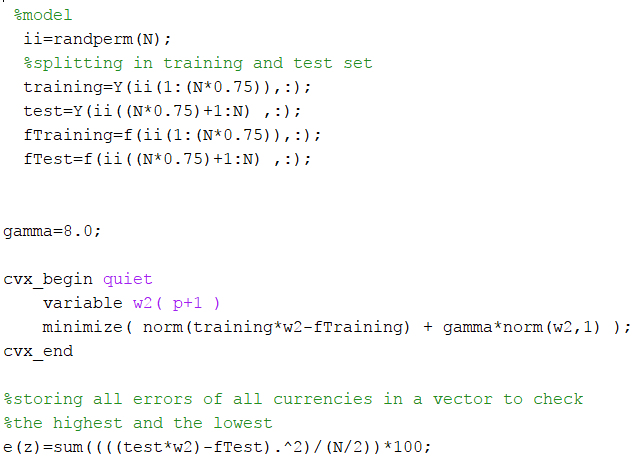
\includegraphics[width=0.4\textwidth]{error.png}
		\caption{Error Calculation}
		\label{error_calc}
	\end{center}
\end{figure}

\iffalse
In the application we have two tables, the top 3 most and the top 3 least predictable exchange rates, which are the currency exchange rates with the lowest and the highest error on the test data respectively.
\fi

\subsection{Consideration about the model}

Depending on the input, the program creates a model to forecast future values. The validity of the model is calculated based on two types of errors : 
\begin{itemize}
\item MAPE (Mean Absolute Percent Error) measures the error in percentage terms. 
\begin{center}
\[ (\frac{1}{N}\sum(\frac{|Actual-Forecast|}{|Actual|}))*100\]
\end{center}
\item MAP (Mean Absolute Deviation) measures the size of the error in units) 
\[ \frac{1}{N}\sum(|Actual-Forecast|\]
\end{itemize}
Both these values, when calculated resulted in producing very low errors (lesser than 1). Which means that our model performed perfectly (with minimal error) when trying to predict the unknow data (test data) using the other currency exchange rate values.
The reasons of that may be numerous:
\begin{itemize}
\item The first reason could be that a lot of currencies were indexed linked with USD and GBP(Eg: the saudi arabia currency) 
\item Influence of major economic trends and activities (i.e. financial cries, economic growth)

\end{itemize}


Justification of the model:
\newline
In the beginning there were some doubts about using regression technique or an ANN(Artificial Neural network)\cite{leung2000forecasting}.
After considering both merits and de-merits, in the end we choose to use linear regression for two reasons : 
\begin{itemize}
\item The main reason was that the ANN is a black box method and it would be very difficult to find any relationship between variables, on the contrary these relationships can be easily shown using regression models. 
\item The method of least squared regression converge much faster than a neural network, and this means saving resources and time 
\end{itemize}

\subsection{Low Frequency data}
The low frequency data included population, employment rate, trade network, GDP, inflation and interest rates from the G-20 countries. Every files downloaded was made in this way (see Fig \ref{raw_eco_data}): 
\newline

\begin{figure}[!h]
	\begin{center}
		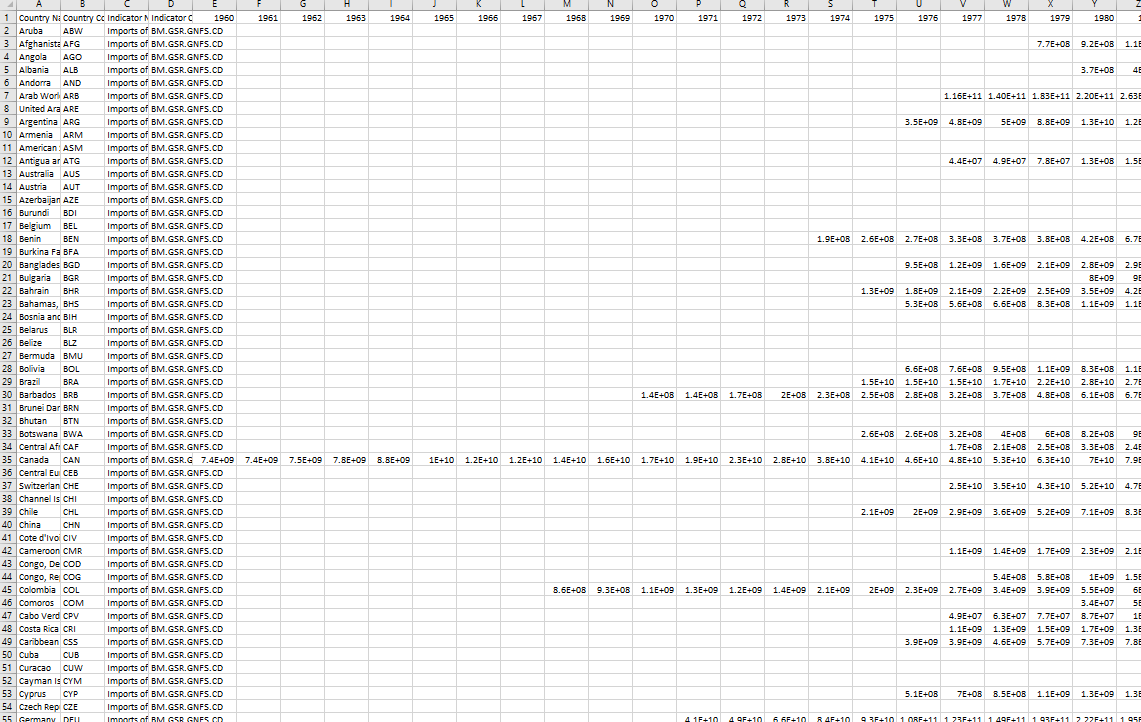
\includegraphics[width=0.40\textwidth]{all_data.png}
		\caption{Raw economic indicators data}
		\label{raw_eco_data}
	\end{center}
\end{figure}

% THIS SECTION BELOW NEEDS SOME MAJOR REWORK, WASN'T ABLE TO UNDERSTAND WHAT THEY DID EXACTLY -- SUMESH
The size of each factor of G-20 dataset table is 265 rows time 61 columns and each row is a country's factor data  from 1960 to 2016.
Firstly, we used python code to select the data of G-20 and used append function to put the G-20 data into a new array.
Then,  in order to clean out the data suitable for using and analysis, we used the zip function to transpose the array.
Next, Due to the low frequency data were analysed from 1991 to 2016, we filtered the data and put it into the new csv file.
Furthermore, we used replace function to remove the space, which may cause the Index error.  Using this python script all low frequency data were filtered and we put the all cleaned data into one file (see Fig \ref{cleaned_eco_data}.
\newline

\begin{figure}[!h]
	\begin{center}
		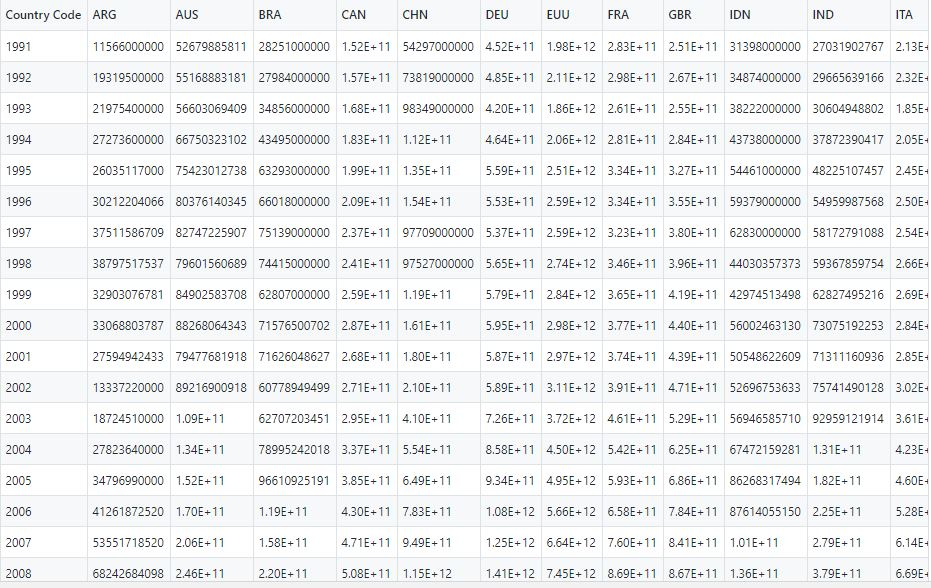
\includegraphics[width=0.40\textwidth]{Capture.JPG}
		\caption{Cleaned Economic data}
		\label{cleaned_eco_data}
	\end{center}
\end{figure}

\subsection{Web Application Design}

We created a simple web application using the python flask framework.
\newline
\newline
The final analysis and displaying of results was implemented in JavaScript and D3
\newline
\newline
When viewing the low frequency economic indicator data we also loaded the high frequency (weekly samples) exchange rate data, this is then aggregated down to yearly samples for analysis with the economic indicators.
\newline
 
\begin{figure}[!h]
	\begin{center}
		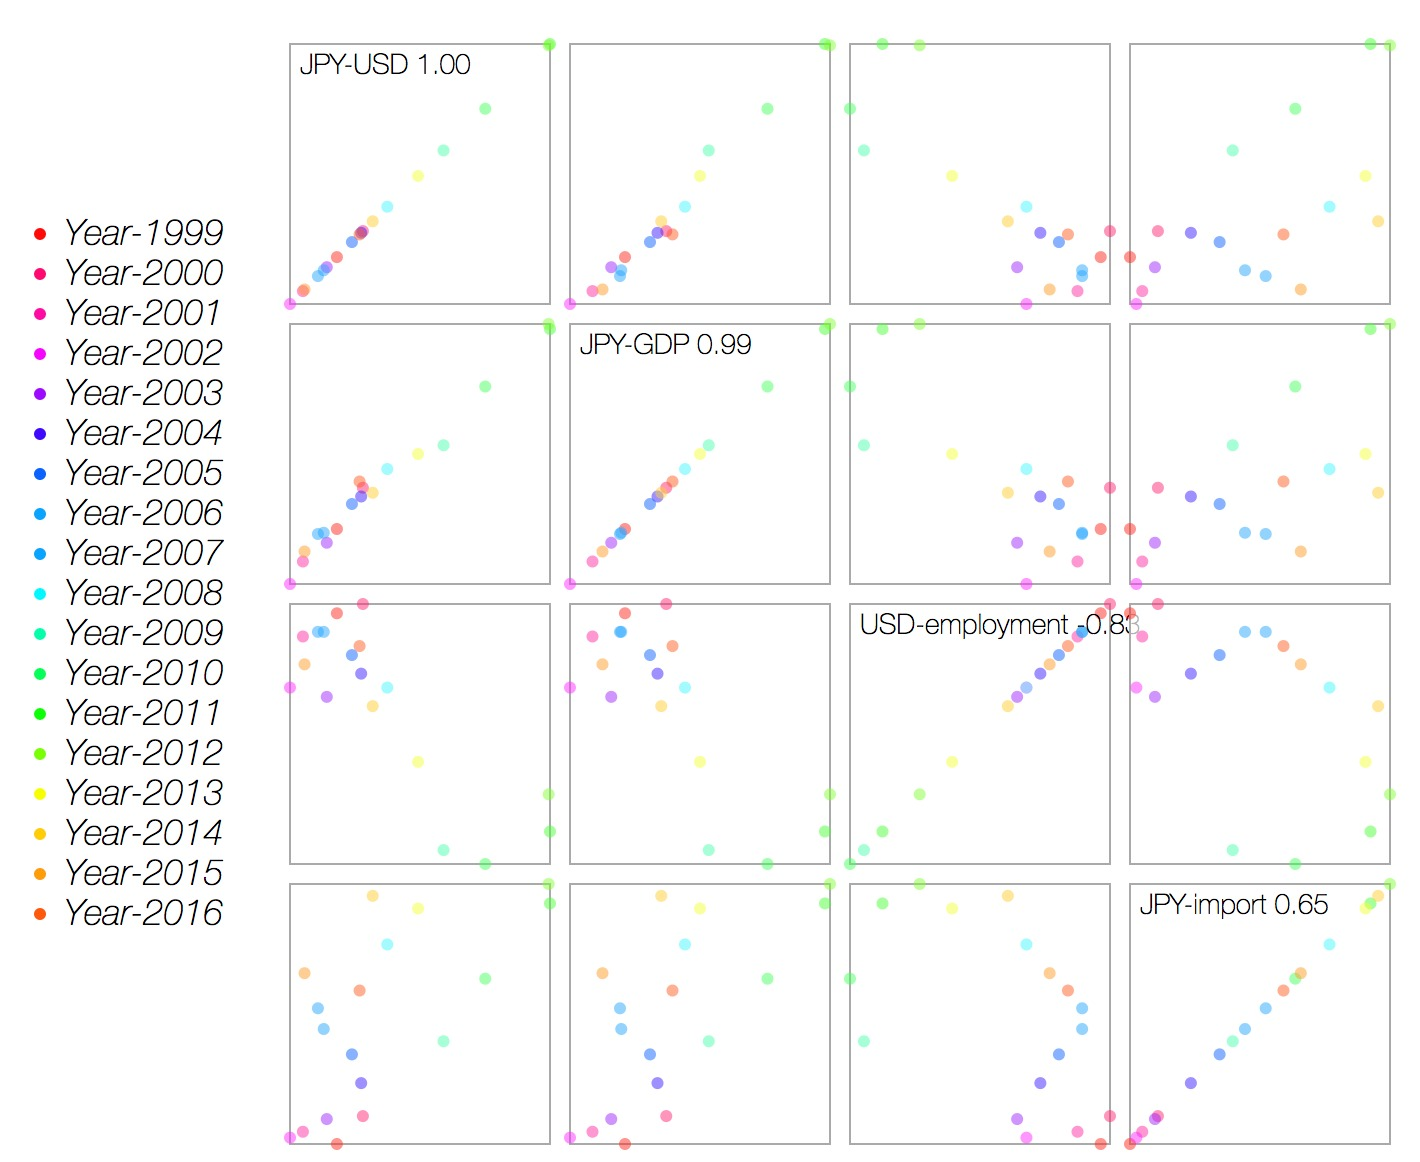
\includegraphics[width=0.30\textwidth]{web.jpg}
		\caption{Covariance Scatter plot of Economic Indicators with respect to a specific exchange rate}
		\label{scatter_plot}
	\end{center}
\end{figure}

The web app has the following two functions:
\newline
\begin{enumerate}
\item Finding Strongest Correlation : When this button is pressed the web app iterates through all the countries currency exchange rates between each other and calculates the correlation coefficient between the exchange rates and their countries respective economic indicator.  This value is then sorted in order of strength (closest to either 1.0 or -1.0) before being displayed.  This allows us to find what are the strongest and weakest correlations. The app then also aggregates the absolute value of each correlation coefficient (to prevent positive and negative correlations cancelling each other out and allowing us to find the average strength of the correlation) with respect to the type of economic indicator.  Which allows us to find the type of economic indicator which is tightly correlated with the exchange rates.

\item Go! : This button takes a selected exchange rate and then generates a scatter plot for each of the economic indicators that are most correlated with those exchange rate. Which is then present in a 4 x 4 grid (as seen in Fig \ref{scatter_plot}), the selected exchange rate is in the top right corner, and each economic indicator is plotted on the diagonal, labelled with their respective correlation coefficient related to the exchange rate.  The user is then able to see a covariance scatter plot for each variable by tracing the horizontal and vertical intersection.
\end{enumerate}

\section{Results}
\subsection{Observation}
As the data we have used is not very huge, we chose to find the strongest correlation between the exchange rates and the indicators which led to this correlation. We have used Pearson's correlation coefficient as a mathematical approach, since the data was not suitable for any sort of mathematical regression or any other kind of predictive analysis. The result that we have found can be summarised below showing the ranking of the indicators in terms of those that are most strongly correlate to  the exchange rate data which are annually averaged over all the exchange rates.
\newline
\begin{itemize}
\item Population = 0.62
\item GDP = 0.60
\item Imports = 0.59
\item Exports = 0.58
\item Foreign Trade = 0.50
\item Inflation GDP Deflator = 0.40
\item Employment = 0.40
\item Interest Rate = 0.40
\item Inflation Consumer Prices = 0.38
\end{itemize}

However in some particular cases we have seen a very strong correlation which are worth mentioning
\begin{table}[!h]
\centering
\caption{Strongest correlation and related indicator}
\label{my-label}
\begin{tabular}{|l|l|l|}
\hline
Currency Code  & Indicator       & Value \\ \hline
JPY-USD        & JPY GDP         & 0.99  \\ \hline
JPY-SAR        & JPY GDP         & 0.99  \\ \hline
SAR-JPY        & JPY GDP         & -0.99 \\ \hline
MXN-CNY        & MXN Population  & -0.98 \\ \hline
AUD-TRY        & TRY Population  & 0.98  \\ \hline
CAD-TRY        & TRY Population  & 0.98  \\ \hline
SAR-CNY        & SAR imports     & -0.98 \\ \hline
AUD-IDR        & IDR Population  & 0.98  \\ \hline
AUD-TRY        & AUD Population  & 0.98  \\ \hline
MXN-CNY        & CNY Population  & -0.98 \\ \hline
RUB-CAD        & CAD Population  & -0.98 \\ \hline
CAD-TRY        & CAD Population  & 0.98  \\ \hline
CNY-SAR        & SAR Imports     & 0.97  \\ \hline
TRY-MXN        & MXN Inflation   & 0.97  \\ \hline
RUB-AUD        & AUD Population  & -0.97 \\ \hline
AUD-IDR        & AUD Population  & 0.97  \\ \hline
AUD-ZAR        & AUD Population  & 0.97  \\ \hline
AUD-ZAR        & ZAR Population & 0.97  \\ \hline
\end{tabular}
\end{table}

From the table above, a few things can be concluded

%IS THIS CONCLUSION DERIVED FROM THE ABOVE TABLE OR SOMEOTHER EXTERNAL SOURCE.?? -- SUMESH
\begin{itemize}
\item Population, GDP and Imports have been the strongest indicators in the past\cite{edwards2006relationship}. These factors have played the most important role in determining the exchange rates for the two currencies
\item A high correlation value indicates that the corresponding indicator is the strongest factor in determining the exchange rates between those two countries\cite{burstein2005large}. For example, We find Japanese GDP has a very strong correlation value (0.99) between Japanese Yen and US Dollar and also between Japanese Yen and Saudi Riyal.  This does not necessarily mean there is a strong correlation, to analysis this we must then look at the covariance scatter plot to understand the relationship and in this case we observe a strong correlation.

% Numzi - can you add results about % error 

\end{itemize}
\subsection{Analysis}
\subsubsection{Currency Exchange Trends}
If we look at the currency exchange rates between Argentina (ARS) and USA (USD) we observe that until 2001 the currency exchange value is 1 and then we see a sudden dip in the value. What could be the reason for this dip? Well, that was because each peso was index-linked to USD at 1ARS= 1USD. However, after the financial crisis of 2001, the fixed exchange rate system was abandoned. Since 2002, the exchange rate started to fluctuate, keeping the exchange rate at between 2.90 and 3.10 pesos per US dollar at that time.  
This is the same case in terms of Saudi Riyal, where even today it is index linked to the USD @ 1 USD = 3.75 SAR 
\subsubsection{Correlation Coefficient}
If we look at the currency exchange rates JPY-USD, we observe that it has a .99 correlation value against the GDP of Japan. Yes, without any arguments we can agree that the GDP of a country has a direct impact on its currency value. Where we saw that the overall influence (correlation coefficient value) of GDP to its countries currency is calculated to be .6. But in this case, we see a value of .99.
\newline
If we look at the history for the currency of Japan (YEN) we see that, following World War II the Yen lost much of its value. To stabilise the Japanese economy the exchange rate of the yen was fixed at 360Yen per 1USD as part of the Bretton Woods system. When that system was abandoned in 1971, the Yen became undervalued and was allowed to float. The Yen had appreciated to a peak of 271Yen per 1 USD in 1973, then underwent periods of depreciation and appreciation due to the 1973 oil crisis, arriving at a value of 227Yen per 1 USD by 1980. Since 1973, the Japanese government has maintained a policy of currency intervention, and the yen is therefore under a "dirty float" regime. This intervention continues until today and that is the reason we see such a tight correlation between the currency exchange of JPY-USD against the GDP of Japan.\newline
But the question is does it stand good for other cases? Well, yes it does? For instance, if we look at the currency of China(CNY) and USA(USD) we see that both these two countries have a relatively huge GDP values, which does have an impact on their respective currencies. But when we look at the exchange rate which is a copula of both these countries currency. There is a possibility that the influence of the GDP values on the exchange rate tend to be slightly lower (Correlation coefficient of China's GDP and US GDP against the exchange rate of CNY-USD is .92 and .87 respectively) but still have a significant impact the exchange rates. 

\section{Conclusion}
\subsection{Economic Indicator}
We have built a tool which allows for the analysis of 254 different exchange rates and their relationship to 9 different economic indicators.  The tool enables you to quickly see for a given exchange rate what are the most correlated economic indicators and visually validate the nature of that correlation.  It also allows you to observe the relationship between the economic indicators them selves.  This can then help guide further investigation into what underlying world events helped drive fluctuations in the exchange rate.

\subsection{Exchange Rate Interrelationships}
% Numzi - Make a statement about what you can use the results for, i.e. something similar to what I have added above.

\section{Limitations and future work}

\begin{itemize}
	\item Limitation : Our data pipeline is not as automated as we would have liked, there is still a significant amount of manual effort required to update our web application with fresh data.
	\begin{itemize}
		\item Improvement : The cleaning we performed was very systematic and with more time could be fully automated in python where the data could be downloaded, clipped and cleaned and finally exported directly the web application.  This would allow the exchange data being used to be refreshed on a daily basis.
	\end{itemize} 
	\item Limitation : The world exchange rates market is very complex and its structure has fluctuated over time. Some of the currencies were index linked to USD prior to 1999, for which we had a limited availability of currency data.  We need to be clear as to the purpose of our tool, our primary aim was to help people understand the relationship between exchange rates and economic indicators and so this is why we deliberately limited or time range so that the user is able to focus on these relationships alone.
	\item Limitation : The dashboard we have created is very limited only focusing on covariance of economic indicators and relative relationships between exchange rates.  This is useful as a tool to help direct further investigation however there is a lot more we could show to support this investigation.
	\begin{itemize}
		\item Improvement : we could expand our dashboard to display all the respective trend date for the correlations that were found.
		\item Improvement : In the exchange rate analysis we could look to automatically find points of inflation in the exchange rate trend data that correlate with the other related exchange rates that were found.  This will identify points in time where something significant might have happened.  Using these time point we could then look to automatically search for financial news related to the countries at those specific time periods.  This would significantly reduce the effort required to explore the economic history of a specific exchange rate.
	\end{itemize}
	
\end{itemize}


% Start of "Sample References" section

% Appendix

% Bibliography
\bibliographystyle{ACM-Reference-Format}
\bibliography{sample-bibliography}



\end{document}
